\documentclass[
	paper=128mm:96mm,% like beamer
	fontsize=11pt,% like beamer
	pagesize ,% write page size to dvi or pdf
	parskip=half -,% paragraphs are separated by half a line
	numbers=noendperiod ,% no periods after section numbers
	captions=nooneline% same treatment of one/several lines
	,bibliography=totoc,listof=totoc, index=totoc,DIV=calc
]{scrartcl}
\linespread {1.12}% enlarge line space
\usepackage[T1]{fontenc}                % Schriftenkodierung
\usepackage[utf8]{inputenc}       % Eingabekodierung Parameter
\usepackage[ngerman]{babel}    % mehrsprachiger Textsatz
\usepackage{fixltx2e}
\usepackage{ellipsis}
\usepackage[tracking=true]{microtype}
\usepackage{lmodern}                        % Ersatz fuer Computer Modern-Schriften
\usepackage{hfoldsty}
\usepackage{fourier}
\usepackage[osf,sc]{mathpazo}
\usepackage{xcolor}
\usepackage{calc}% working with lengths , counters etc.
\usepackage[includeheadfoot, top=3.5mm, bottom=3.5mm, left=5.5mm, right=5.5mm, headsep=6.5mm, footskip=8.5mm]{geometry}% set page layout parameters
\usepackage{scrpage2}% package for page style with not only uppercase letters in the head
\usepackage{titlesec}% for reducing space between ((sub)sub)sections and text
\usepackage{tocstyle}% for adjusting table of contents
\usepackage{mathtools}
%\usepackage{units}
%\usepackage{siunitx} % Benutzung: \SI{1}{\metre}
\usepackage{bm}
\usepackage{enumitem}
\usepackage{graphicx}
\usepackage{wrapfig}
%\renewcommand{\scriptsize}{\tiny}
%\usepackage[format=plain, labelformat=default, textformat=period, justification=centering, font=scriptsize, labelfont=bf]{caption}
%\captionsetup[figure]{name=Abb.}
%\captionsetup[wrapfigure]{name=Abb.}
%\captionsetup[wrapfigure]{margin=10pt}
\usepackage{framed} % usage: \begin{framed}  ... \end{framed}
\usepackage{tikz}
\usepackage{tabularx}
\usepackage{booktabs}
\usepackage{multicol}
%\usepackage[numbers,square,comma,sort&compress,merge]{natbib}
\usepackage{url}
\usepackage[hidelinks%citebordercolor=white,linkbordercolor=white,urlbordercolor=white,
%,pdfpagemode=FullScreen%
]{hyperref}

\definecolor{mybgcolor}{HTML}{002F2F} %Colors: 002F2F, 046380, EFECCA, A7A37E, E6E2AF
\definecolor{mybgcolor2}{HTML}{EFECCA}
\definecolor{mydotcolor}{HTML}{046380}
\definecolor{mydotcolor2}{HTML}{A7A37E}
\definecolor{myfontcolor1}{HTML}{E6E2AF}
\definecolor{black}{rgb}{0,0,0}
\definecolor{shadecolor}{rgb}{255,0,0}

\pagecolor{mybgcolor2}

\newcommand{\mycbox}[1]{\tikz{\path[draw=#1,fill=#1] (0,0) rectangle (4pt,4pt);}}

\newcommand{\mytitle}{Bericht des StAPF}
\newcommand{\myauthor}{StAPF}
\newcommand{\myuni}{St\"andiger Ausschuss der Physik-Fachschaften}
\newcommand{\mydate}{27. Mai 2015}

% page style
\pagestyle{scrheadings} % activates pagestyle from scrpage 2
\clearscrheadfoot % clear head and foot
\setkomafont{pageheadfoot}{\large\color{myfontcolor1}\sffamily}% setting for page head and foot
% optical vertical centering of page contents
\makeatletter
\renewcommand*{\@textbottom}{\vskip \z@ \@plus 1fil }
\newcommand*{\@texttop}{\vskip \z@ \@plus .5fil }
\addtolength{\parskip}{\z@ \@plus .25fil} % stretch parskip
\makeatother

\ihead{ % head left
	\hspace{-2mm}%
	\begin{tikzpicture}[remember picture, overlay]
	\node[xshift=\paperwidth/2, yshift=-\headheight] (mybar) at (current page.north west)[rectangle,fill,inner sep=0pt, minimum width=\paperwidth,minimum height=2\headheight, top color=mybgcolor!64, bottom color=mybgcolor]{}; % bar
	\node[below of=mybar,yshift=3.3mm, rectangle, shade,inner sep=0 pt, minimum width=128mm, minimum height=1.5mm, top color=black!50, bottom color=myfontcolor1]{}; %shadow
	\end{tikzpicture}%
	\Large{\textbf{\mytitle}}
}

%\newlength{\footheight}
\setlength{\footheight}{8mm}
\addtokomafont{pagefoot}{\footnotesize} % size for foot
\setkomafont{pagenumber}{\color{myfontcolor1}} % white page number
\ifoot{% foot left
	\hspace{-2mm}%
	\begin{tikzpicture}[remember picture,overlay]
		\node[xshift=\paperwidth/2, yshift=\footheight/2] at (current page.south west)[rectangle, fill, inner sep=0pt, minimum width=\paperwidth, minimum height=\footheight, top color=mybgcolor!64, bottom color=mybgcolor]{}; % bar
	\end{tikzpicture}%
	\myauthor\ \raisebox{0.2mm}{$\bm{\vert}$}\ \myuni
}
\ofoot[\pagemark\hspace{-2mm}]{\pagemark\hspace{-2mm}}%foot right ( plain pages do also have page numbers )

\AtBeginDocument{\renewcaptionname{ngerman}{\contentsname}{Gliederung}}% change name of toc
\makeatletter
\newtocstyle[noonewithdot]{nodotnopagenumber}{% define tocstyle without dots and page numbers
	\settocfeature{pagenumberbox}{\@gobble}%
}
\makeatother
\usetocstyle{nodotnopagenumber}
%\setcounter{tocdepth}{2}
%\renewcommand*{\sectionmarkformat}{}
%\renewcommand*{\subsectionmarkformat}{}
\titlespacing*{\section}{-30pt}{0pt}{0pt}
%\titlespacing*{\subsection}{0pt}{0pt}{0pt}
%\titlespacing*{\subsubsection}{0pt}{0pt}{0pt}
%\titleformat{\section}{\color{white}\tiny}{}{0pt}{}
%\addtokomafont{subsubsection}{\large}
%\addtokomafont{subsection}{\Large}

%\automark[section]{\mytitle}

%\include{command}

\begin{document}
\thispagestyle{empty}
\begin{tikzpicture}[remember picture,overlay]
 \path [top color = mybgcolor!64,bottom color = mybgcolor] (current page.north east)rectangle (current page.south west);
\end{tikzpicture}
{\color{myfontcolor1}
	\begin{flushright}
%		\vspace{-0.5cm}
		{\Huge \textbf{\textsf{\mytitle}}}\\
		\vspace{.5cm}
		{\LARGE Sommer-ZaPF 2015 in Aachen}\\
		\vspace{.5cm}
		{\LARGE \mydate}
	\end{flushright}
}

%\tableofcontents
\pagebreak
\addsec{Aktuelle Zusammensetzung: \O ~HS-Sem. \(= 11.2\)}
	\begin{itemize}[label=\mycbox{mydotcolor}]
	    \item \emph{Bj"orn Guth (RWTH Aachen)} (Sprecher)
		\item \emph{Margret Heinze (LMU M"unchen)}
		\item \emph{Csongor Keuer (TU Berlin)	}	
		\item Lea Meyer (Uni Kiel)
		\item Niklas Luhmann (Uni Konstanz)
	\end{itemize}
	\textbf{IM Lobachewsky:} J\"org Behrmann \\
	\textbf{Nebenrolle:} Adriana Röttger
\pagebreak

\addsec{Öffentlichkeitsarbeit}
	\begin{itemize}[label=\mycbox{mydotcolor}]
		\item allg. keine Resolutionen aus Bremen
		\item Veröffentlichung vom Bericht
		\item Fehlendes Protokoll vom Endplenum 
		\item Studienführer
	\end{itemize}

\addsec{Studieneingangstest - Mathematische Vorkenntnisse}
	\begin{itemize}[label=\mycbox{mydotcolor}]
		\item Andreas Borowski wurde eingeladen um über den Stuieneingangstest, der von ihm zum WiSe 2013/14 durchgeführt wurde zu berichten. (Wurde bereits in Bremen angekündigt)
	\end{itemize}

\addsec{IT-Infrastruktur}
	\begin{itemize}[label=\mycbox{mydotcolor}]
		\item Server wurde zum Teil schon aufgesetzt 
		\item AK auf dieser ZaPF
		\item Organisation und Arbeit im Wiki / Studienführer
	\end{itemize}

\pagebreak
\addsec{Akkreditierungspool}
	\begin{itemize}[label=\mycbox{mydotcolor}]
		\item 17 Personen im \emph{Programmakkreditierungspool},\\ 2 Personen im \emph{Systemakkreditierungspool}
		\begin{itemize}[label=\color{mydotcolor2}$\pmb\rightarrow$]
			\item Verl"angerung der Entsendung:\quad \emph{Markus Gleich (FU Berlin), Margret Heinze (LMU), Bj\"orn Guth (RWTH Aachen), Ioannis Caltzidis (Uni Stuttgart), Jakob Schnell (Uni Heidelberg) \& Thomas Kirchner (Uni Heidelberg)}
		\end{itemize}
		\item 34. PVT in Kaiserslautern (20.03. - 22.03.2015)
		\item nächstes PVT 
	\end{itemize}
\pagebreak
\begin{center}
	\begin{framed}
		{{\Huge \textsf{\textbf{Wichtig}}} \\~\\ \Large Neue Anmeldeformulare f\"ur den Pool ausf\"ullen und in digitaler Form an die Verwaltung senden!}
	\end{framed}
\end{center}
\pagebreak
\addsec{MeTaFa}
	\begin{itemize}[label=\mycbox{mydotcolor}]
		\item physisches Treffen in Halberstadt (26.09. - 28.09.2014)
		\begin{itemize}[label=\color{mydotcolor2}$\pmb\rightarrow$]
			\item Themen: neues BAföG, Richtlinien des Akkreditierungspools
		\end{itemize}
		\item n\"achstes Treffen in Aachen (20.03. - 22.03.2015) \emph{(in Planung)}
	\end{itemize}
\addsec{Kontakt zu anderen BuFaTas}
	\textbf{Zu Gast bei:}
	\begin{itemize}[label=\mycbox{mydotcolor}]
		\item BuFaTa Geographie
		\item KoMa
	\end{itemize}
	\textbf{Termine anderer BuFaTas:}
	\begin{itemize}[label=\mycbox{mydotcolor}]
		\item zeitgleich: Philosophie (B), Biologie (AC)
		\item PsyFako (27.11. - 30.11.14, MR)
	\end{itemize}

\addsec{Doktorandika-Umfrage}
	\begin{itemize}[label=\mycbox{mydotcolor}]
		\item Verantwortlicher: \emph{J\"org}
		\item 898 Teilnehmende (768 Online)
		\item Auswertung abgeschlossen
		\item Vorstellung in AK \& Zwischenplenum
%		\begin{itemize}[label=\color{mydotcolor2}$\pmb\rightarrow$]
%			\item
%		\end{itemize}
	\end{itemize}

\addsec{Doktorandika-Umfrage}


\pagebreak
\renewcommand{\mytitle}{Bericht des KommGrem}
\renewcommand{\myauthor}{KommGrem}
\renewcommand{\myuni}{Kommunikationsgremium \textit{zwischen jDPG und ZaPF}}
\addcontentsline{toc}{section}{Kommunikationsgremium}
\section*{Aktuelle Zusammensetzung}
	\begin{itemize}[label=\mycbox{mydotcolor}]
		\item ZaPF:\quad \emph{Margret Heinze (LMU M"unchen) \& \\  Daniela Kern-Michler (Uni Frankfurt)}
		\item jDPG: \quad \emph{Hejo Kerl (ETH Z"urich) \& \\ Sebastian Heupts (Uni Heidelberg)}
	\end{itemize}
\section*{Sprecherschaft}
	\begin{itemize}[label=\mycbox{mydotcolor}]
		\item Sprecherin: \quad \emph{Margret Heinze (ZaPF)}
	\end{itemize}
\pagebreak
\section*{Berichte der letzten beiden KFP-Sitzungen}
	\begin{itemize}[label=\mycbox{mydotcolor}]
		\item 10.06.-11.06.14 (Bad Honnef) \& 02.11.14 (Berlin)
	\end{itemize}
	\textbf{Themen:}
	\begin{multicols}{2}
		\begin{itemize}[label=\color{mydotcolor2}$\pmb\rightarrow$]
			\item Online-Mathe-Br\"uckenkurs
			\item Vergleich der Mathematikkenntnisse von Studienanf\"angern 1970 und Heute
			\item CHE-Hochschulranking
			\item KFP-Studierendenstatistik
			\item Promotionsstudie der DPG
			\item Studienatlas Physik
			\item Sprecherschaft der KFP
		\end{itemize}
	\end{multicols}

\section*{Bachelor-/Master-Umfrage}
	\begin{itemize}[label=\mycbox{mydotcolor}]
		\item Umfrage im letzten Semester an 33 Fachbereichen durchgef\"uhrt
		\item Beginn der Auswertung
		\begin{itemize}[label=\color{mydotcolor2}$\pmb\rightarrow$]
			\item Nachbefragung
		\end{itemize}
		\item AK \& weitere Infos im Zwischenplenum
	\end{itemize}
\section*{CHE-Hochschulranking}
	\begin{itemize}[label=\mycbox{mydotcolor}]
		\item Umfrage l\"auft aktuell
	\end{itemize}
		\textbf{Was bisher geschah:}
		\begin{itemize}[label=\color{mydotcolor2}$\pmb\rightarrow$]
			\item Frageb\"ogen im Wesentlichen unver\"andert
			\item Gespr\"ach mit der ZEIT: Einigung für Online-Darstellung, Printversion schwierig
		\end{itemize}
		\textbf{Perspektive:}
		\begin{itemize}[label=\color{mydotcolor2}$\pmb\rightarrow$]
			\item Treffen von Task-Force und CHE im Januar 2015
		\end{itemize}

\addsec{Aktueller Stand: Indikatoren}
\begin{multicols}{2}
		\begin{itemize}[label=\color{mydotcolor2}$\pmb\rightarrow$]
			\item Studieneinstieg
			\item Lehrangebot
			\item Laborpraktika
			\item Studierbarkeit
			\item Betreuung
			\item Kontakt unter Studierenden
			\item Räume
			\item IT Ausstattung
			\item \emph{Wissenschaftsbezug, Auslandsaufenthalte, Internationale Ausrichtung}
			\item Anteil Absolventen in Regelstudienzeit + 1 Sem.
			\item Unterstützung zum Studieneinstieg
		\end{itemize}
\end{multicols}
\pagebreak
\addsec{Vorschlag zur Darstellung}
%\begin{center}
%	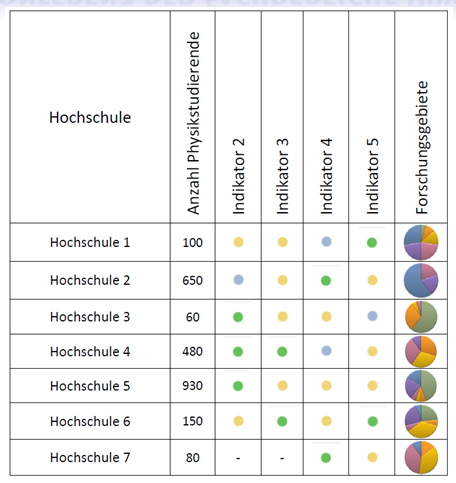
\includegraphics[height=0.85\textheight]{KFP_CHE_Forschungsprofil.PNG}
%\end{center}

\pagebreak
\thispagestyle{empty}
\begin{tikzpicture}[remember picture,overlay]
 \path [top color = mybgcolor,bottom color = mybgcolor!64] (current page.north east)rectangle (current page.south west);
\end{tikzpicture}
{\color{myfontcolor1}
	\begin{center}
%		\vspace{-0.5cm}
		{\Huge \textbf{Fragen? Anregungen? ...}}\\
	\end{center}
}
\end{document}
